%%% Notes on Single stellar population production of N %%% 

\documentclass[12pt]{report} 
\usepackage{hyperref} 
\usepackage{float} 
\usepackage{natbib}
\usepackage{amsmath} 
\usepackage{amssymb} 
\usepackage{caption}
\usepackage{float}
\usepackage[export]{adjustbox} 
\usepackage[margin = 1in]{geometry} 
\hypersetup{
	colorlinks 		= true,
	urlcolor 		= blue,
	linkcolor 		= blue, 
	citecolor 		= blue
}

\newcommand\mnras{MNRAS} 
\newcommand\apj{ApJ} 
\newcommand\apjs{ApJS} 
\newcommand\aap{A\&A} 
\newcommand\araa{ARA\&A} 
\newcommand\twolineskip{\par\noindent\null\par\noindent} 
\newcommand{\ddfrac}[2]{\frac{\displaystyle #1}{\displaystyle #2}} 

\begin{document} 
\begin{center} 
\textbf{{\Large Single Stellar Population Production of Nitrogen}} \\ 
James W. Johnson 
\end{center} 

\noindent 
{\Large \textit{Production Timescales Relative to Fe}} 
\par\noindent 
Using~$y_\text{N}^\text{CC} = 5\times10^{-4}$, the AGB star yields of N from 
the FRUITY database~\citep{Cristallo2011}, and supernova yields of Fe as in 
\citet{Johnson2020} and~\citet{Weinberg2017} (i.e.~$y_\text{Fe}^\text{CC}$ = 
0.0012 and~$y_\text{Fe}^\text{Ia}$~= 0.0017),~\textbf{what is the net 
production of N and Fe as a function of stellar population age and 
metallicity?} 
\par 
Figure~\ref{fig:n_vs_fe_ssp} shows the net production of N and Fe as a function 
of stellar population age and metallicity. Since Fe has metallicity-independent 
yields under these assumptions, it's plotted with only one curve, whereas N has 
different production timescales at different metallicities. In general, the 
CCSN yields of N under these assumptions make up a substantially larger 
fraction of the N production than the CCSN yields of Fe does for its 
production. This means that the characteristic timescales for N production are 
significantly shorter than for Fe. 
\par
The AGB yields of N are also significantly weighted toward high masses such 
that even at solar metallicity,~$\gtrsim$90\% of the N production is complete 
by the time the population is~$\tau$~= 1 Gyr old. Although the fractional 
yields are higher for more massive AGB stars, this does not mean that the 
total N produced in low-mass AGB stars is lower than that produced by high mass 
AGB stars due to the steep nature of the initial mass function. In a window of 
progenitor mass [$m$,~$m + dm$] at a metallicity~$Z$, the total mass of N 
produced is given by: 
\begin{equation} 
dm_\text{N} = y(m|Z)m\frac{dN}{dm} = y(m|Z)\xi m^{1 - \alpha} 
\end{equation} 
where~$\alpha$~is the power-law index of the IMF. If the production at two 
masses~$m_1$~and~$m_2$~are comparable, then the scaling of the yield~$y$~with 
progenitor mass can be derived: 
\begin{subequations}\begin{align} 
dm_\text{N}|_{m = m_1} &= dm_\text{N}|_{m = m_2} \\ 
\implies y(m_1|Z) \xi m_1^{1 - \alpha} &= y(m_2|Z) \xi m_2^{1 - \alpha} \\ 
\implies \frac{y(m_1|Z)}{y(m_2|Z)} &= \left(\frac{m_1}{m_2}\right)^{\alpha - 1} 
\end{align}\end{subequations} 

\begin{figure}[t] 
\centering 
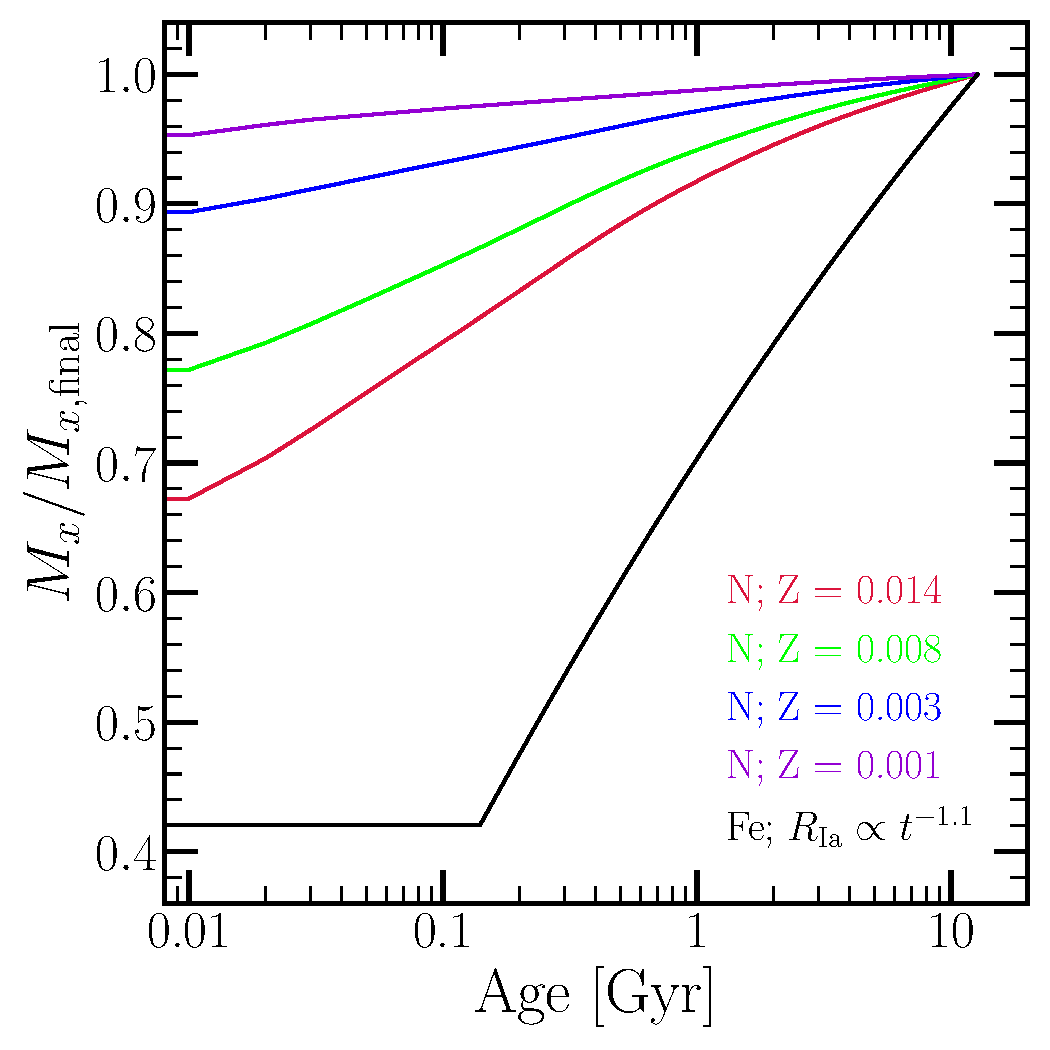
\includegraphics[scale = 0.5]{n_vs_fe_ssp.pdf} 
\caption{Net mass of N (colored lines) and Fe (black) as a function of stellar 
population age and metallicity (color-coded according to legend for N), in 
units of the mass produced at~$\tau$~= 12.2 Gyr. } 
\label{fig:n_vs_fe_ssp} 
\end{figure} 

This demonstrates that if the IMF-integrated mass production of any element in 
AGB stars is to be mass-independent, then the yield must scale with 1 less than 
the power-law index of the IMF at masses of~$M \gtrsim 1~M_\odot$. If the IMF 
has a slope of~$\alpha$~= 2.3 at these masses, then the yield must scale with 
$m^\beta$~where~$\beta \geq$~1.3. Any higher, and the IMF-integrated net 
production is more biased toward high mass stars, and conversely toward low 
mass stars for lower values of~$\beta$. Based on these investigations of the 
\citet{Cristallo2011} yields (see~\texttt{../yields/yields.pdf}), it appears 
that~$\beta \approx$~1 for nitrogen, indicating the IMF-integrated production 
is actually dominated by low-mass stars. 
\twolineskip 
{\Large \textit{How can the production be dominated by high-mass stars if the 
IMF-integrated yields are dominated by low-mass stars?}} 
This appears to be due to the long lifetimes of low mass stars. It's one thing 
for low mass stars to contribute significantly to a given yield, but only 
those with lifetimes on the order of a hubble time or shorter are going to 
enrich the ISM. 

\newpage 
\bibliographystyle{mnras} 
\bibliography{ssp} 

\end{document} 

